\chapter{TINJAUAN PUSTAKA}

\section{Tinjauan Pustaka}
\subsection{Teknologi Pelacak}
Penelitian sebelumnya telah mengembangkan berbagai sistem pelacak aset dengan berbagai macam pendekatan pada perangkat keras maupun perangkat lunak untuk berbagai aplikasi. Sebagai contoh, \cite{Ekhsan2022} merancang suatu sistem untuk melacak dompet dengan menggunakan TK-102 GPS \textit{Tracker}.

Tim peneliti dari \textit{Vidyalankar Institute of Technology} telah merancang suatu sistem yang dapat mendeteksi lokasi dari kendaraan dan juga emisi \ce{CO} yang dihasilkan. Pada sistem yang dirancang, digunakan \textit{development board} Arduino Uno yang berbasis mikrokontroler ATmega328. Ketika kandungan gas \ce{CO} sudah melebihi ambang batas, sistem akan memutus pengiriman bahan bakar dan kemudian mengirimkan data koordinat dari modul GPS ke \textit{server} Apache yang telah dirancang \cite{Asha2022}.

Sebuah sistem \textit{speedometer} telah dirancang oleh \cite{Najmurrokhman2021}. Sistem tersebut menggunakan modul GPS untuk menghitung kecepatan dan koordinat lokasi kendaraan. Data kecepatan kendaraan didapat dari menghitung waktu yang dibutuhkan oleh kendaraan untuk berpindah dari satu titik ke titik lainnya. Data yang didapat dikirimkan dengan API Adafruit IO menggunakan modul SIM808.

Penelitian yang dilakukan oleh \cite{Mukhtar2015} dari \textit{University of London} menggunakan mikrokontroler AT89S52 dari keluarga 8051. Digunakan modul GPS M-89 yang diatur untuk menerima isyarat transmisi satelit pada frekuensi 1575.42 MHz. Data yang diterima akan ditampilkan pada layar LCD dan dikirimkan dengan modul GSM. Kemudian, data yang telah diterima akan ditampilkan pada situs web.

\subsection{Transmisi Data Nirkabel}


Sistem dapat dikembangkan dengan banyak cara, tetapi pada penelitian ini sistem yang akan dirancang hanya fokus untuk melacak lokasi dari kendaraan, dalam kasus ini adalah bus kampus "Trans Gadjah Mada"

\section{Dasar Teori}
\subsection{STM32 Nucleo-WL55JC1}
STM32 Nucleo-WL55JC1 adalah \textit{development board} berbasis mikrokontroler STM32WL55 yang  dikembangkan oleh ST Microelectronics. Mikrokontroler yang digunakan adalah STM32WL55  \textit{dual-core }Arm Cortex-M4/M0+ dengan \textit{clock speed} 48 MHz \cite{STMicroelectronics2022a}.

\begin{figure}[ht]
	\centering
	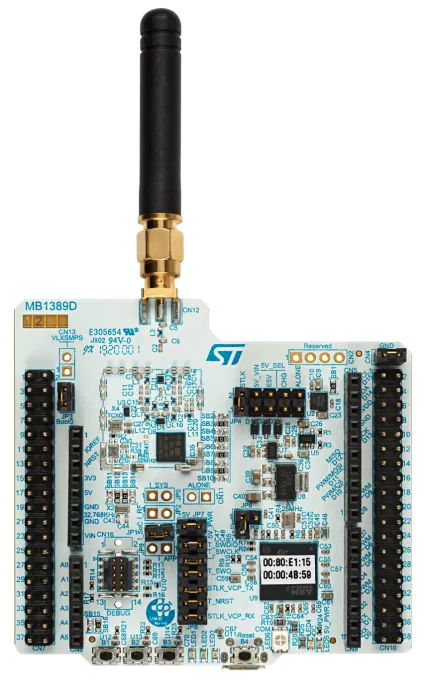
\includegraphics[width=5cm]{contents/chapter-2/stm32-wl55jc1.jpg}
	\caption{\textit{Development Board} STM32 Nucleo-WL55JC1}
	\label{Fig: STM32 Nucleo-WL55JC1}
\end{figure}

Perangkat ini sudah terintegrasi dengan STLINK-V3E, sehingga tidak dibutuhkan perangkat tambahan untuk memrogram dan melakukan \textit{debugging} pada perangkat \cite{STMicroelectronics2022}. Selain itu, perangkat ini juga mendukung penggunaan \textit{expansion board} Arduino dan ST morpho. \textit{Development board} STM32 Nucleo-WL55JC1 ditunjukan oleh Gambar \ref{Fig: STM32 Nucleo-WL55JC1}.

Mikrokontroler STM32WL55 memiliki \textit{clock speed} 48 MHz jika dibandingkan dengan Arduino Mega yang hanya 16 MHz. Selain itu, STM32WL55 memiliki SRAM dengan kapasitas 64 KB atau delapan kali lipat dari yang dimiliki oleh Arduino Mega \cite{STMicroelectronics2022b}.

Karena performa tinggi dengan konsumsi daya rendah, maka digunakan mikrokontroler STM32WL55. Selain itu, STM32 juga memiliki komunitas yang tidak kalah luas dengan komunitas Arduino dan ESP-32.

\subsection{Modul GNSS Teseo LIV3FL}
\subsection{Antena GPS }
\subsection{Modul LoRa(?)}